\documentclass[conference]{IEEEtran}
% RSS 2027 Stage 1 extended abstract (5 pages content + 1 page references). Anonymous. Template: RSS IEEEtran 1.7a.
% Numbers: docs/note/analysis_note_draft.md and data_results/*/summary.md (ledger docs/LEDGER.md). Simulation only.
\usepackage{times}
\usepackage[numbers]{natbib}
\usepackage{multicol}
\usepackage[bookmarks=true,hidelinks]{hyperref}
\usepackage{graphicx}
\usepackage{booktabs}
\usepackage{amsmath,amssymb}

\pdfinfo{
   /Author (Anonymous)
   /Title  (Shadows Bias Feature-Field Object Trackers Through an Implicit Silhouette Term)
   /Subject (Robot perception)
   /Keywords (object tracking; Gaussian splatting; feature fields; evaluation)
}

\begin{document}
\title{Shadows Bias Feature-Field Object Trackers\\Through an Implicit Silhouette Term}
\author{Author Names Omitted for Anonymous Review. Paper-ID [add your ID here]}
\maketitle

\begin{abstract}
Robots increasingly track objects by rendering a Gaussian splat with distilled DINO features and matching it to
the live image. Such trackers report high recovery rates for tools under perturbation. We re-implement one of them,
POGS, in a simulator with exact ground truth, and find that its published recovery rule leaves roll about the tool
axis free and hides a systematic roll error of $9.5\pm2.8^\circ$ that is present before any perturbation. Under a
full rotation rule recovery falls from 17--39 to 2--14 of 50 trials, and a relative rule is passed by a tracker that
never moves. The error is not an optimisation failure: the loss itself prefers the wrong pose. We trace it to an
implicit silhouette term inside the region-of-interest feature loss, which compares background pixels with an empty
render. Its pose gradient is a boundary term that rewards silhouettes covering high-norm live features; a
pre-registered test shows that this term predicts the sign of the bias in all 48 strongly biased conditions and its
rank across 60 (Spearman 0.80), mostly through how much background a rotation uncovers rather than where the shadow
lies. On three independently trained splats the roll minimum
follows the gripper's shadow strength (Spearman $\rho\le-0.85$, shifts of 5--9$^\circ$), a rendered background removes
the dependence, and the objective of a second tracker (RSRD) shows the same bias. Pre-registered tests refute our own
first explanation, that the term supplies the restoring force, and six corrections fail a criterion fixed in
advance. We propose evaluation rules with a reference implementation, and an extension plan: the official code, real
captures with a controlled lamp, and an explicit shadow-free silhouette term.
\end{abstract}

\IEEEpeerreviewmaketitle

\section{Introduction}
Persistent feature fields let a robot track an object it has scanned once. A Gaussian
splat~\cite{kerbl2023gaussian} is distilled with DINO features~\cite{oquab2024dinov2}; at run time the pose of each
object group is optimised so that its rendered features match the features of the live
image~\cite{kerr2024rsrd,yu2025pogs}. POGS~\cite{yu2025pogs} uses this to grasp and servo tools, and reports 48 of 50
drill recoveries for perturbations up to $15^\circ$ and 40 of 50 at $30^\circ$.

Feature matching is attractive because DINO features are thought to be insensitive to lighting. We show that the
way the loss is \emph{assembled} undoes part of that robustness. The loss is a mean over a region of interest (ROI)
around the object, but the prediction is an object-only render. Every background pixel is therefore compared with
zero, and the loss contains a silhouette term in disguise. Region-based trackers optimise such terms explicitly and
are known to be sensitive to shadows and background clutter~\cite{prisacariu2012pwp3d,stoiber2022srt3d}; feature-field
trackers inherit the sensitivity without stating it.

\textbf{Problem.} Why does a feature-field tracker that recovers well under a published rule carry a persistent
rotation error, and what part of its objective causes it? \textbf{Hypotheses.}
\textbf{H1} (evaluation): the published rule frees exactly the DOF in which the tracker is biased.
\textbf{H2} (mechanism): the bias is carried by the background part of the ROI loss, not by the object features.
\textbf{H3} (cause): the bias follows the cast shadow in a dose-dependent way, on independently trained splats and in
a second tracker's objective. \textbf{H4} (a hypothesis we held and tested): the background term supplies most of the
static restoring force, which would explain why removing it breaks tracking.

\textbf{Contributions.} (1)~An evaluation finding with a null-model check (H1). (2)~A mechanism: an implicit
silhouette term, a first-order analysis of its pose gradient tested by a pre-registered prediction, and
term-by-term evidence (H2). (3)~A shadow
dose-response replicated on three splats and in RSRD's objective (H3). (4)~Negative results with criteria fixed in
advance: H4 is refuted and six corrections fail. (5)~Evaluation rules with code. All tests after the initial
diagnosis were pre-registered in timestamped documents before any result existed.

\section{Related work}
\textbf{Feature-field tracking.} RSRD~\cite{kerr2024rsrd} recovers part motion from monocular video by optimising
part poses of a DINO-embedded splat; POGS~\cite{yu2025pogs} adds object grouping and persistent tracking with depth
for manipulation. Both average a feature loss over the ROI with the object-only render as the prediction.
Analysis-by-synthesis pose estimation with radiance fields began with iNeRF~\cite{yen2021inerf}; Gaussian-splat
trackers with photometric or mask objectives include 6DOPE-GS~\cite{jin20246dope} and GSGTrack~\cite{gsgtrack2024}.
\textbf{Region-based tracking.} PWP3D~\cite{prisacariu2012pwp3d} and SRT3D~\cite{stoiber2022srt3d} move a projected
silhouette so that it separates foreground and background statistics; their pose gradients are boundary integrals.
We show that a feature-field loss contains such a term implicitly and that this term, not the object features,
carries the shadow bias. \textbf{Evaluation.} Pose errors that are ambiguous under symmetry or free DOF are discussed
in~\cite{hodan2016evaluation}; we add the case of a rule that frees the DOF in which a method is biased.

\section{Setting}
We re-implement the POGS release: splatfacto-style training (4000 steps) with DINOv2 ViT-S/14 features reduced to 64
dimensions by PCA, contrastive grouping, and per-frame tracking by Adam on a 7-DOF group pose (25 iterations) with an
ROI DINO $L_2$ loss and an optional depth term. A simulator renders a tool scene (a procedural drill on a table among
five household objects) with exact ground truth: a 35-view capture, three splats trained with different seeds
(train-view PSNR 33.5--33.6\,dB), and an in-grasp protocol after the paper: approach, grasp, lift, rotate by
$\pm15^\circ$ or $\pm30^\circ$, return; 50 seeds per setting. Every result table includes \emph{Static}, the initial
pose never updated.

\section{H1: the recovery rule hides a roll bias}
POGS scores a trial as recovered when the tool tip is within 3\,cm and the bit-axis direction within $5^\circ$; roll
about the bit axis is left free~\cite{yu2025pogs}. Table~\ref{tab:rules} scores the same trajectories under this rule,
under a full rotation rule, and for Static.
\begin{table}[t]\centering\caption{In-grasp recovery out of 50 by rule. Paper: 48 ($\le15^\circ$), 40 ($30^\circ$).}\label{tab:rules}
\begin{tabular}{lccc}\toprule
Setting & Full rotation & Roll-free (paper) & Static (both)\\\midrule
$+15^\circ$ & 2 & 32 & 0\\ $-15^\circ$ & 14 & 25 & 0\\ $+30^\circ$ & 13 & 39 & 0\\ $-30^\circ$ & 5 & 17 & 0\\\bottomrule
\end{tabular}\end{table}
Under the paper's rule we reproduce its $30^\circ$ result in one direction (39 vs.\ 40, Fisher $p=1.0$) and fall short
elsewhere ($p\le10^{-4}$). Under the full rule recovery collapses. 94\% of the pre-perturbation rotation error is roll
about the bit axis ($|\text{roll}|=9.5\pm2.8^\circ$, swing $4.0\pm3.4^\circ$, Fig.~\ref{fig:roll}); it is already
$12.5^\circ$ at the end of the approach, before the gripper touches the drill. The signed pre-perturbation error
about the perturbation axis is positive in 167 of 200 trials, so a $+$ perturbation moves the truth toward the biased
estimate and a $-$ one away from it, which explains why $+$ settings recover more often. A post-hoc relative rule
(``back to the pre-perturbation error'') is passed by Static in 7--9 of 21--29 trials when the perturbation aligns
with this error and never (0 of 21--29) when it opposes it. A Kalman motion prior does not change any of this: a filter models zero-mean scatter, not a bias.
\begin{figure}[t]\centering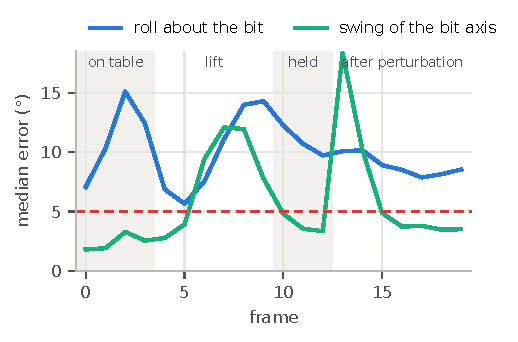
\includegraphics[width=\linewidth]{figs/o4_roll_trace.pdf}
\caption{Median roll about the bit axis and swing of the axis over the in-grasp trials (200 trials). The roll error
exists before the perturbation.}\label{fig:roll}\end{figure}

\section{H2: an implicit silhouette term}\label{sec:mechanism}
\textbf{Decomposition.} Let $e(p)=\lVert f(p)-\hat f_\theta(p)\rVert$ be the feature residual at pixel $p$ of an ROI
$\Omega$ with $N$ pixels, where $f$ are live features and $\hat f_\theta$ the blurred object-only render at pose
$\theta$, with rendered mask $M(\theta)$:
\begin{align}
L(\theta)&=\tfrac1N\textstyle\sum_{p\in\Omega} e(p)=S_\text{in}(\theta)+S_\text{out}(\theta),\\
S_\text{out}(\theta)&=\tfrac1N\textstyle\sum_{p\notin M(\theta)} e(p)\;\approx\;\tfrac1N\textstyle\sum_{p\notin M(\theta)} g(p),\nonumber
\end{align}
with $g(p)=\lVert f(p)\rVert$.
Off the object the render is near zero, so $S_\text{out}$ is the summed norm of the live features that the predicted
silhouette leaves uncovered. In the drill ROI 87\% of pixels are background.

\textbf{Pose gradient.} Treating the ROI as continuous and writing $v_n(x)=\langle\partial x/\partial\theta,
n(x)\rangle$ for the outward normal velocity of the silhouette boundary $\partial M$ under a pose change, the
transport theorem gives
\begin{equation}
\frac{\partial L}{\partial\theta}=\frac1N\oint_{\partial M}\bigl(e_\text{in}(x)-g(x)\bigr)\,v_n(x)\,ds
+\frac1N\int_{M}\frac{\partial e}{\partial\theta}\,dx, \label{eq:grad}
\end{equation}
with $e_\text{in}$ the residual just inside the boundary. The first term is the region-competition flow of
PWP3D-style trackers: the silhouette expands where the live background has a larger feature norm than the object
residual and contracts elsewhere. Rotating an asymmetric object such as a drill about its axis covers background
on one side and uncovers it on the other, by unequal amounts; the term therefore produces a torque that grows with
the feature norm of the surrounding background, and a cast shadow changes that norm. With the object term locally
quadratic and unbiased, the minimum moves to $\hat a=-T/(2\kappa)$, where $T$ is the derivative of the background part
at the true pose and $\kappa$ the curvature of $L$. Replacing the empty render by a render of the static background
replaces $g$ by $\lVert f-\hat f_\text{bg}\rVert$, which is small wherever the background is unchanged, and removes the
torque from unchanged regions.

\textbf{Test of Eq.~\eqref{eq:grad} (pre-registered, E4).} We computed $T$ from the live features and the soft rendered
silhouette alone, $B(\theta)=\frac1N\sum_p(1-\alpha_\theta(p))\,g(p)$, at $\pm1^\circ$, and compared $\hat a$ with the
measured minimum in 60 conditions (three splats; six shadow strengths with the gripper, two frames without it, 12
held-out views). The prediction ranks the measured bias (Spearman $0.80$, rule $\ge0.5$, pass) and has the correct sign
in all 48 conditions with $|a|\ge2^\circ$ (rule $\ge75\%$, pass; Fig.~\ref{fig:torque}); it overestimates the magnitude
by about $2\times$, as expected from a first-order term that ignores the blur of the render. A third rule fails: a
predictor that keeps only the change of uncovered area, with $g$ replaced by its ROI mean, does almost as well
(Spearman $0.76$; required gain $\ge0.2$, observed $0.04$). The bias is therefore driven mainly by how much background
a rotation uncovers, weighted by the overall feature norm that the shadow sets, not by where the shadow lies.
\begin{figure}[t]\centering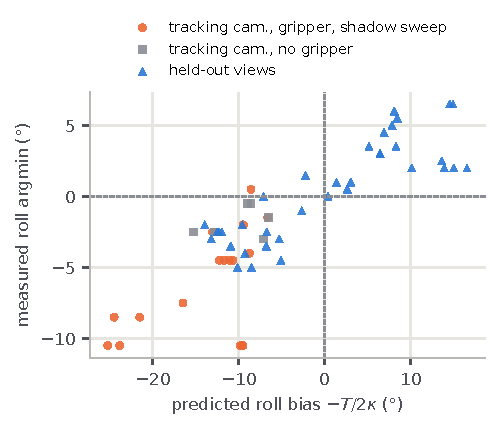
\includegraphics[width=\linewidth]{figs/torque_scatter.pdf}
\caption{Pre-registered test of the boundary term: predicted roll bias $-T/2\kappa$ from live features and the
rendered silhouette alone vs.\ measured roll argmin, 60 conditions on three splats.}\label{fig:torque}\end{figure}

\textbf{Evidence (term by term, at the true pose).} (i)~The ground truth is exact: RGB-only argmins lie within
$0.5^\circ$ and 0.5\,mm of it in all 8 sweeps. (ii)~The object features are unbiased:
restricted to the true-pose mask, the DINO minimum is within $1^\circ$ of the truth in all 16 views. (iii)~The full ROI
minimum sits at $-10^\circ$ at the tracking camera with the gripper's shadow, $-6^\circ$ without the gripper and $-2^\circ$
with shadows off (Fig.~\ref{fig:argmin}). (iv)~With a rendered background instead of an empty one the minimum moves
from $-10^\circ$ to $+2^\circ$, and the held-out-view mean $|$argmin$|$ falls from $3.7^\circ$ to $1.3^\circ$.
\begin{figure}[t]\centering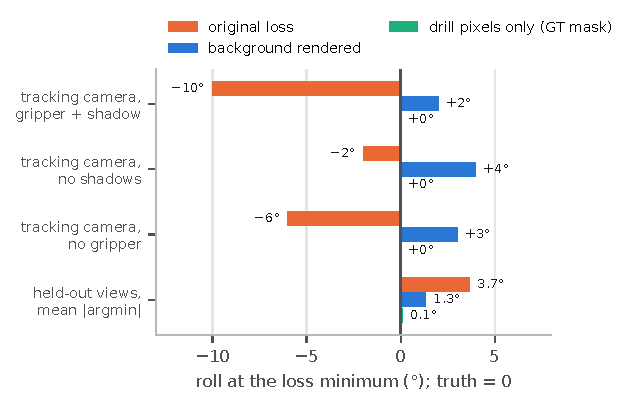
\includegraphics[width=\linewidth]{figs/finding_argmin.pdf}
\caption{Roll at the minimum of each loss term, drill at the true pose, across views and lighting.}\label{fig:argmin}\end{figure}

\section{H3: a shadow dose-response that replicates}\label{sec:g1}
We pre-registered five predictions before any sweep: three splats of the tool scene trained with different seeds;
four objects (drill, mug, mustard bottle, cereal box); the tracking camera with and without shadows and 12 held-out
views; rotations about three axes. For the dose-response only the tracking frame is re-rendered, with the cast-shadow
factor $1-s(1-0.22)$, $s\in\{0,0.25,\dots,1.25\}$; the splats were trained at $s=1$.
\begin{figure}[t]\centering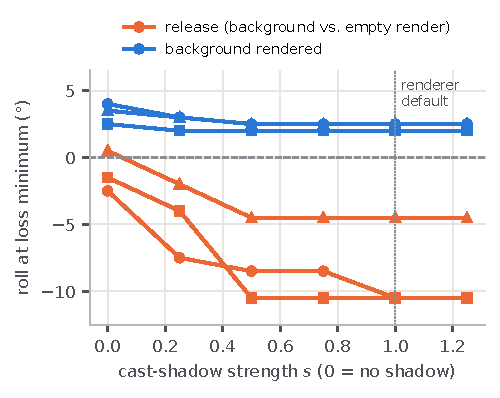
\includegraphics[width=\linewidth]{figs/dose_response.pdf}
\caption{Roll at the minimum of the DINO loss vs.\ cast-shadow strength, drill at the true pose, gripper at its
frame-0 pose, three independently trained splats (markers).}\label{fig:dose}\end{figure}
\begin{table}[t]\centering\caption{Pre-registered generality results (static sweeps), in the order fixed in advance.}\label{tab:g1}
\small\begin{tabular}{@{}p{0.6\linewidth}p{0.33\linewidth}@{}}\toprule Prediction & Result\\\midrule
P1: background carries $>50\%$ of the local rotational curvature ($\geq3$/4 objects; drill on new splats) & fail (2/4; drill 0.10, 0.17, 0.27)\\
P2: drill roll bias $\leq-5^\circ$ replicates on new splats & pass ($-10, -10, -5^\circ$)\\
P3: rendered background lowers mean $|$argmin$|$ on held-out views ($\geq3$/4) & fail (2/4)\\
P4: monotone shadow dose-response, shift $\ge4^\circ$ ($\geq2$/3 splats) & pass (3/3)\\
P5: rendered background moves $<$ half as much ($\geq2$/3) & pass (3/3)\\\bottomrule
\end{tabular}\end{table}
The bias and its shadow dependence replicate (Table~\ref{tab:g1}, Fig.~\ref{fig:dose}): Spearman $\rho=-0.97,-0.85,
-0.85$ and shifts from $s=0$ to $s=1$ of $-8.0^\circ$, $-9.0^\circ$, $-5.0^\circ$, while the rendered-background loss
moves by 0.5--1.5$^\circ$ and stays at $+2$ to $+4^\circ$. In line with Eq.~\eqref{eq:grad}, the background torque $T$
increases with $s$ (exploratory; Spearman 1.00, 1.00, 0.66 on the three splats). P3 fails: the rendered background removes the shadow dependence but
not every view-dependent offset. A further pre-registered test bounds the claim: without the gripper, scaling only
the scene's own cast shadows moves the minimum by $\ge2^\circ$ with $|\rho|\ge0.8$ for one of four objects (the mug) on at
least two splats (rule: three of four; fail). The dose-response therefore needs a shadow that covers a large part of
the ROI, as an occluding gripper's does; small self-shadows of tabletop objects barely move the minimum.

\textbf{A second tracker's objective.} RSRD~\cite{kerr2024rsrd} builds its DINO loss the same way (object-only render,
sharp inside the mask and blurred outside, averaged over the ROI) and adds an RGB term over the ROI, also against
the object-only render. Its objective, evaluated with our splats and renderer (pre-registered), places the drill's
roll minimum with the gripper's shadow at $-10^\circ$, the same as POGS. RSRD and POGS share code lineage, so this
tests the objective family, not an independent implementation.

\section{H4 refuted, and six corrections that fail}\label{sec:fixes}
\textbf{H4.} Removing the background breaks tracking: DINO restricted to the per-pose object mask recovers 1/0/4/4 of
25 trials vs.\ 9/12/16/23 for POGS. We expected the background to supply the restoring force. Three pre-registered
static tests say otherwise: near the truth the object features provide most of the rotational curvature for the
drill (P1: background share 0.10--0.27) and 75--100\% of the translational stiffness for every object, and a
rendered background is 1.4--1.6 times as stiff as the release loss. The trajectory failure of the masked variants is
translation drift during the lift. A pre-registered sweep along the true lift trajectory (120 frames in which
the gripper holds the drill) does not explain it either: at the true pose the masked objective is no more biased in
translation than the release objective (median 6.0 vs.\ 6.0\,mm) and not flatter. The failure is dynamic, arising
from estimate-dependent masks and ROIs, not from the objective at the true pose.

\textbf{Corrections.} The pass rule was fixed before the runs: a paired roll-free bootstrap CI above zero in at least
2 of 4 settings and below zero in none, lower pre-perturbation roll, and better than a depth-only control in at least
2 settings.
\begin{table}[t]\centering\caption{Corrections: roll-free recoveries out of 25 ($-30/-15/+15/+30^\circ$).}\label{tab:fixes}
\begin{tabular}{lcc}\toprule Variant & Recoveries & Pass\\\midrule
Static (no motion) & 0/0/0/0 & --\\
POGS (release) & 9/12/16/23 & ref.\\
RGB term, weight 1 & 16/13/20/18 & no\\
Depth $\times30$ & 2/1/0/0 & no\\ Depth $\times100$ & 0/0/0/0 & no\\
DINO inside object mask & 1/0/4/4 & no\\ DINO vs.\ rendered background & 0/0/0/0 & no\\
Depth only (DINO off) & 0/0/0/0 & control\\\bottomrule\end{tabular}\end{table}
Heavier depth halves the roll but fits the gripper once it occludes the drill. Re-distilled features (DINOv2 with
registers, DINOv3 ViT-S/16, feature upsampling) fail on held-out views before any trajectory is run. The rendered
background removes the bias on static frames but is stale once the object moves. The bias is a property of the
objective's construction; changing its weights or its features does not remove it.

\section{Evaluation rules}\label{sec:recs}
(1)~Report the full and the tool-axis rule side by side and state which DOF a rule frees. (2)~Score every rule on a
no-motion baseline; avoid relative rules, or stratify them by the sign of the pre-existing error. (3)~Store full
SE(3) per frame and decompose the error into roll and swing about the tool axis. (4)~Before attributing an error to
observability, sweep the loss at the true pose term by term across views and lighting. A reference implementation
produces all four in one call and will be released.

\section{Planned extensions (proposed Extension Charter)}
Each extension has a written protocol with pass rules fixed before data is seen.
\textbf{E1: official code.} Train and track with the official POGS code on the same capture and repeat the roll and
dose-response sweeps (OR1: roll minimum $\le-5^\circ$ with the gripper's shadow; OR2: $\rho\le-0.8$ and a shift
$\ge4^\circ$; OR3: agreement with our implementation across 13 views). A failure narrows the claim to our
implementation and will be reported as such.
\textbf{E2: real captures.} A drill on an AprilTag board scanned under diffuse light; test frames at three tripod
viewpoints with one lamp at controlled positions and intensities and an occluder that casts a shadow into the ROI.
The drill never moves, so the scan pose is the ground truth. Predictions: R1 roll minimum $\le-5^\circ$ (same sign as in
simulation); R2 the object-mask loss removes more than half of it; R3 shadow-in-ROI frames shift the minimum by
$\ge4^\circ$ relative to shadow-free frames (bootstrap CI excluding zero). A photometric shadow measure, computed from
images only, gives the dose axis.
\textbf{E3: an explicit, shadow-free silhouette.} Replace the implicit term by a depth-foreground silhouette with the
gripper's known geometry excluded, evaluated on held-out seeds against the same rule and a reference that receives
the same exclusion.
\textbf{E4: beyond first order.} The first-order term ranks and signs the bias but overestimates it; we will add the
blur of the render near the boundary and test the corrected magnitude on held-out splats.
\textbf{E5: the dynamic failure.} Static sweeps at the true pose, at frame 0 and along the lift, do not explain
the masked tracker's drift; we will test the feedback between the estimate-dependent mask and the ROI by tracking
with masks frozen at the true pose versus at the estimate.

\section{Limitations}
All results so far are simulated, with one lighting model; real cameras add exposure changes and sensor noise. The
dose-response is established for the drill under a gripper's shadow (three splats of one scene); scene self-shadows
alone do not reproduce it for most objects.
The second tracker is RSRD's objective in our framework, not the RSRD code. Eq.~\eqref{eq:grad} is first-order and
ignores the blur of the render near the boundary. The $\pm$ asymmetry of recovery is not explained by the mechanism
alone: a depth-only tracker shows it too.

\bibliographystyle{plainnat}
\bibliography{refs}
\end{document}
